% 第 10 周交付物：S&P 500 股票池、批量流水线、优化前后对比与面板理论线（中文版）—— 编译方式：XeLaTeX
\documentclass[11pt]{ctexart}
\usepackage[a4paper, margin=2.2cm]{geometry}
\usepackage{amsmath, amssymb}
\usepackage{booktabs}
\usepackage{graphicx}
\usepackage{float}
\usepackage[hidelinks]{hyperref}
\usepackage{enumitem}
\setlist{nosep}
\usepackage{parskip}

\title{\textbf{S\&P 500 股票池、批量流水线与面板检验}\\
\large Chooser Option 定价项目 · 第 10 周（Enhancement 第 2 周）}
\author{佟铸城（Zhucheng Tong）}
\date{2026 年 9 月 29 日}

\begin{document}
\maketitle

\section{本周目标与完成情况}

第 10 周把第 9 周的单票在线骨架扩到指数成分股，并按导师"补充实验"的要求把优化做出来、给出优化前后的倍数。同时兑现两条承诺：向量化批量定价路径本周接上；S\&P 500 日更压到分钟级。

\begin{center}\small
\begin{tabular}{p{4.0cm}p{11.0cm}}
\toprule
目标 & 完成情况 \\
\midrule
股票池 & 点时（point-in-time）S\&P 500 成员：2018 年至今 666 只标的、670 段成员区间；任意日期成员数 505--509；590 只有价格历史，76 只为 Yahoo 无历史的已退市标的 \\
多源采集 & yfinance 批量 $\to$ yfinance 单票 $\to$ Alpha Vantage 三级回退，指数退避重试；Stooq 因反爬被排除 \\
批量流水线 & 增量拉取按所需窗口分组、增量特征重建、一次向量化全池定价与情景；590 只日更实测 38 秒 \\
向量化定价 & \texttt{quote\_universe} / \texttt{scenario\_universe}，与单票标量路径逐位一致（审计 4、5） \\
优化实验 & 五组优化前后对比（E1--E5），倍数 5.4 到 164 \\
前端 & 新增"全市场概览"页签：578 只已定价标的、行业汇总 \\
理论线 & GARCH 期限结构锚在 497 只标的上复检；锚定残差 ML 第一轮（面板、walk-forward、测试集封存） \\
自检 & 十项审计全过（含第 9 周八项回归） \\
\bottomrule
\end{tabular}
\end{center}

\section{股票池：点时成员的构造}

来源是 Wikipedia 的 S\&P 500 成分表与"历史变更"表，均为公开可再分发的清单。Wikipedia 在 2026 年把变更表从页面移除，本周从最后一个仍含该表的修订版（2026-05-23）读取，其后的变化由当前表的"加入日期"与两次快照的差集推断。从今日集合逆向回放 395 条变更，得到每只标的的成员区间 $[\text{start},\text{end})$。校验：今日点时集合与当前成分表完全相等，每只标的的区间互不重叠，JPM 全程在池，四个探针日期成员数 509/508/505/505。

如实记录的局限：（1）代码更名（如 FB $\to$ META）在来源中记为一删一增，看起来像两只标的；（2）2018--2020 年被剔除且已退市的 76 只标的在 Yahoo 无历史，训练面板对这段时间带有部分生存偏差，比例与名单已写入审计 8 的输出；（3）Alpha Vantage 免费档只提供未复权价，仅作最后回退并在来源列标记，本周实际未触发（590 只全部来自 yfinance 批量）。

\section{批量流水线与优化实验}

\subsection{改动}

\begin{itemize}
  \item \textbf{采集}：按每只标的所需窗口分组批量下载（新标的拉全史，其余拉 10 天重叠），一个陈旧标的不再把整批的窗口拉宽。
  \item \textbf{特征增量重建}：18 个特征最长回看 504 行（股息同比 = 252 日滚动和的 252 日变化），取尾部 760 行重算、只回写末尾 40 行；EWMA 锚是无限记忆的递推，从切换行的存量值播种，$v_t=\lambda v_{t-1}+(1-\lambda)r_t^2$ 给定种子即精确。审计 2 证明增量与全量逐位一致（$10^{-14}$）。
  \item \textbf{状态落库}：\texttt{sigma\_ewma} 与 \texttt{r\_1y\_dev} 随特征入库，报价只读最新一行（PostgreSQL \texttt{DISTINCT ON}），不再拉全段历史。
  \item \textbf{向量化定价}：全池报价一次数组闭式解，参考模型对特征矩阵一次预测，情景表同样向量化。
  \item \textbf{稳健性}：多标的暴露了单票看不到的问题——无分红或首次分红标的的股息同比出现 $0/0$ 与 $+\infty$，坏价格行使 Parkinson 波动率为无穷，特别分红使股息率达 228\%。处理：股息同比在上年为零时定义为 0，Parkinson 仅对正价格计算，定价用的股息率上限 25\%（原始值保留在库中），非有限输入的标的从批次剔除而不拖垮整批。JPM 的文件特征逐位不变（第 9 周审计 1）。
\end{itemize}

\subsection{优化前后（同一进程、同一硬件下复测"前"路径，倍数与硬件无关）}

硬件：Apple M4 Pro（14 核）、24 GB。

\begin{center}\small
\begin{tabular}{p{0.9cm}p{6.6cm}rrr}
\toprule
编号 & 实验 & 优化前 & 优化后 & 倍数 \\
\midrule
E1 & 单票特征重建：全量 2190 行重算回写 / 增量 40 行 & 436 ms & 45.8 ms & 9.5$\times$ \\
E2 & 报价的市场状态加载：全段历史 + 推导 / 读最新一行 & 17.9 ms & 2.6 ms & 6.8$\times$ \\
E3 & 全池报价 578 只：逐票标量路径（外推） / 向量化 & 2217 ms & 412 ms & 5.4$\times$ \\
E4 & 全池情景表 578 只：逐票 / 向量化 & 414.5 ms & 2.5 ms & 164$\times$ \\
E5 & 日更流水线 590 只：第 9 周单票 4.5 s 串行外推 / 本周批量实测 & 2654 s & 38.0 s & 70$\times$ \\
\bottomrule
\end{tabular}
\end{center}

E5 的分段耗时：市场指数与利率 12.8 s、股票价格批量拉取 9.0 s、特征增量重建 14.7 s、全池报价 0.9 s、缓存失效 0.2 s。三点读数：（1）"分钟级"承诺已兑现，且是秒级；（2）剩余大头是网络（指数、利率四个串行请求）与逐票特征重建（590 次小查询与写入），是第 12 周的候选；（3）E3 只有 5.4 倍，向量化定价本身不到 1 ms，412 ms 几乎全在 \texttt{DISTINCT ON} 扫 124 万行特征表——加一个 \texttt{(ticker, date DESC)} 索引或维护"最新行"物化视图是明确的下一步。

\section{审计（十项，全部通过）}

\begin{center}\small
\begin{tabular}{p{0.8cm}p{7.8cm}p{6.4cm}}
\toprule
编号 & 断言 & 结果 \\
\midrule
1 & 成员区间一致：今日集合 == 当前表、无重叠、JPM 全程、探针计数 & 666 只、509/508/505/505 \\
2 & 增量特征 == 全量重建（JPM + 4 只随机） & 最大差 $1.2\times10^{-14}$ \\
3 & 落库的 EWMA / 利率偏差 == 全段推导 & 最大差 $1.1\times10^{-16}$ \\
4 & 向量化报价 == 单票标量报价（全部字段） & 最大差 $2.8\times10^{-14}$ \\
5 & 向量化情景 == 单票情景表 & 差 0 \\
6 & 全池每只标的 $\max(C,P)\le$ chooser $\le$ straddle；误差带 == 第 4 周分状态 MAE & 578 只通过（1 只触发股息率上限） \\
7 & 批量流水线幂等（重算两次报价不变） & 通过 \\
8 & 价格覆盖率 $\ge 95\%$ 当前成分股，缺失名单与原因列出 & 当前 503 只覆盖 100\%；76 只历史成员无价格（已退市） \\
9 & 第 9 周八项审计回归 & 通过 \\
10 & 理论线测试集封存：实际用到的训练数据截止日 $<$ 测试起始日 & 训练数据止 2023-03-08（净化后），测试起 2024-03-21 \\
\bottomrule
\end{tabular}
\end{center}

两条审计自身的修正值得记录。（a）审计 6 初版用严格不等式，AIV 因股息率 228\% 使 call 腿为零、chooser 与 put 在浮点精度上相等而失败——这不是套利，改为带 $10^{-9}$ 容差的 $\le$，并引出上述股息率上限。（b）第 9 周审计 1 与 5 在本周失败：Yahoo 在每次分红后重算\textbf{整段}复权收盘价，本地文件快照与在线库是两个数据版本，跨版本比对特征不是在检验代码。改为"用第 2 周文件管道在库内价格上重算，与库内特征比对"（同版本、逐位一致），并把版本差作为信息打印；历史报价行是当日的审计留痕，只断言最新一行可复现。

\section{理论线 A：GARCH 期限结构锚在面板上的复检}

第 9 周在 JPM 上，GARCH(1,1) 一年期限结构锚综合分 0.804。本周同一协议（每 21 日重估、$\ge750$ 观测、参照为各标的自己的 EWMA、第 4 周 8 指标综合分）跑遍点时成员：面板 617{,}211 行、532 只标的（2019-10-17 至 2024-12-31），497 只有足够行数计算综合分。

\begin{center}\footnotesize
\begin{tabular}{lrrrrrr}
\toprule
锚 & 胜率（综合分$<1$） & 综合分中位 & 四分位 & 池化 MAE & 池化 Bias & 池化综合分 \\
\midrule
EWMA（参照） & -- & 1.000 & -- & 7.87 & $-2.49$ & 1.000 \\
GARCH 1 年期限结构 & 54.5\% & 0.952 & 0.665--1.436 & 7.32 & $+3.81$ & 0.980 \\
GARCH 1 日 & 72.2\% & 0.906 & -- & 6.88 & $-0.53$ & 0.812 \\
\bottomrule
\end{tabular}
\end{center}

\begin{figure}[H]
\centering
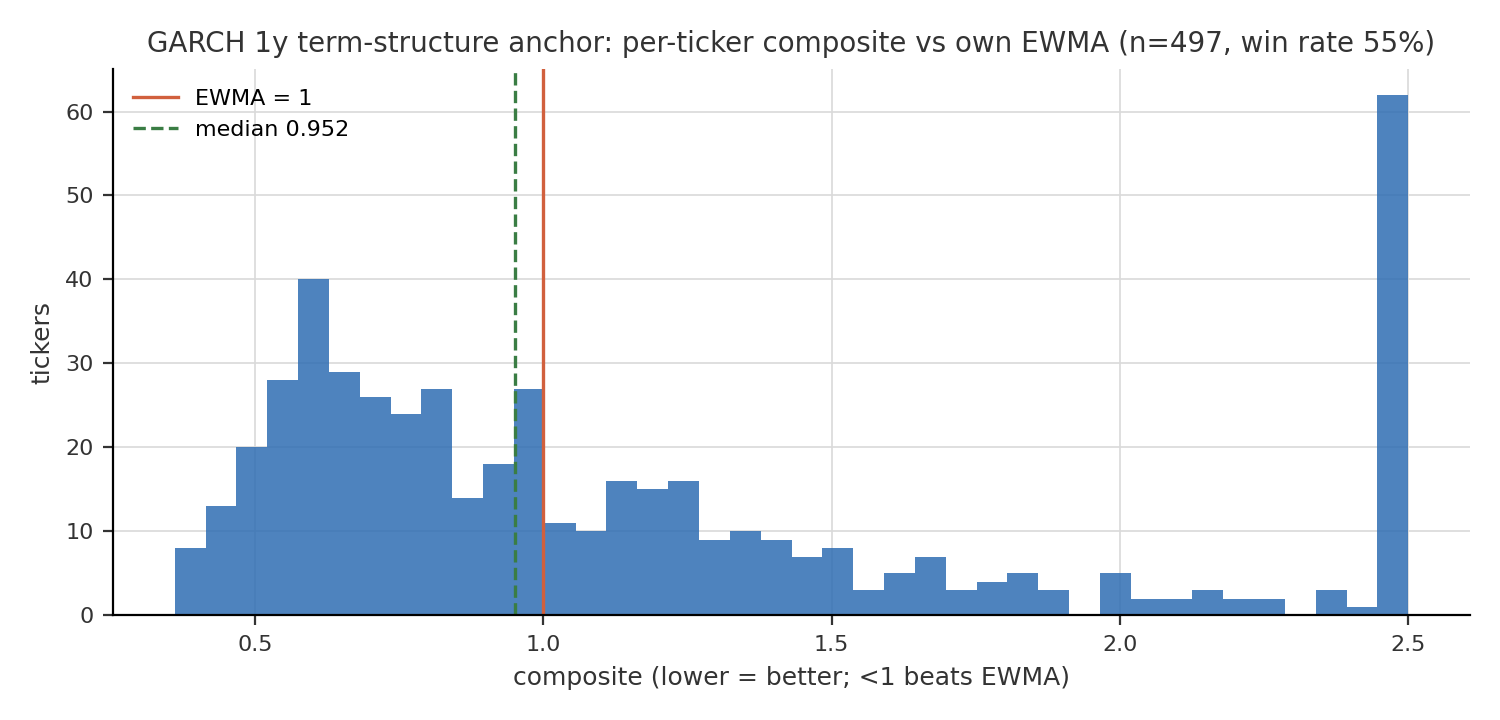
\includegraphics[width=0.9\textwidth]{figures/garch_panel_composite_hist.png}
\caption{每只标的的 GARCH 1 年锚综合分（对自身 EWMA）：双峰——约 0.6 的一大群与 $>2.5$ 的 60 只长尾}
\end{figure}

\textbf{读数}：JPM 上的 0.804 在面板上没有站住。1 年锚的胜率 54.5\%、中位 0.952，接近掷硬币；分布双峰，长尾 60 只标的的持续性 $\alpha+\beta$ 中位 0.968（整体 0.943）且全部正偏差（中位 $+5.99$ 美元）——持续性越接近 1，长期方差水平估得越不稳，期限结构平均就把一个错误的水平"做满"。分状态它在恐慌期明显更好（6.32 对 8.49），平静期持平（7.59 对 7.70）；分年 2020 与 2023 明显更差。反而是不做期限结构平均的 GARCH 1 日锚更稳：胜率 72\%、池化综合分 0.812、偏差接近零。结论：\textbf{不换锚}。工具主定价维持 EWMA；GARCH 1 日锚作为第 11 周的第二候选，1 年期限结构锚只在持续性远离 1 的标的上有意义，这是一个可检验的门控条件。

\section{理论线 B：锚定残差学习第一轮（面板）}

目标 $y=\ln(\sigma_{oracle}/\sigma_{EWMA})$，第 6 周 16 特征，按\textbf{日期}做 70/15/15 净化切分（训练止 2023-06-07，验证 2023-06-08 至 2024-03-20，测试 2024-03-21 起\textbf{封存}），验证期内按季度 walk-forward 重训，每块只用截至块起始日前 253 个交易日的数据。验证集 95{,}345 行、494 只标的。

\begin{center}\small
\begin{tabular}{lrrrrrr}
\toprule
模型 & MAE(\$) & Bias & P95AE & Hit10 & 综合分 & 分标的胜率 \\
\midrule
EWMA（参照） & 6.10 & $-1.96$ & 22.2 & 30.6\% & 1.000 & -- \\
锚定 Ridge & 27.66 & $+27.4$ & 81.4 & 2.2\% & 7.159 & 1.2\% \\
锚定 Ridge（特征 1/99 分位截尾） & 23.46 & $+23.1$ & 69.6 & 2.8\% & 6.124 & 2.2\% \\
锚定 GBDT & 10.63 & $+9.6$ & 33.1 & 12.5\% & 2.225 & 18.3\% \\
GARCH 1 年锚（同一验证窗） & 8.64 & $+7.2$ & 25.5 & 17.3\% & 1.692 & -- \\
\bottomrule
\end{tabular}
\end{center}

\textbf{读数}：全部劣于 EWMA，而且方向一致——系统性\textbf{高估}。训练窗以 2020--2022 为主，面板层面的标签均值（oracle 高于 EWMA）被模型学成常数项，验证窗 2023--24 是低波动期，修正量整体偏正。截尾只把 Ridge 从 7.16 改善到 6.12，说明失败主因不是横截面离群值，而是\textbf{时间上的分布漂移}，与第 5 周单票时的失败是同一个机制，只是样本从 1 只变成 494 只并没有消除它——扩大截面不能替代更长的时间历史。第二轮（第 11 周）的修改方向由此确定：按日期对目标与特征做横截面去均值（学"相对同日其他标的"的修正，而不是绝对水平）、加入标的固定效应或行业哑变量、以 GARCH 1 日锚替代 EWMA 锚重做，并保持测试集封存到第 11 周只开一次。

\section{工具中的 ML 参考价：一个必须标注的边界}

概览页初版对 578 只标的都给出了 ML 参考价，但参考模型是第 6 周仅用 JPM 训练并封存检验的锚定 Ridge。对其他标的这是分布外外推：43 只标的的修正比率触到 $\pm1.5$ 的裁剪边界，196 只超过 $\pm0.5$；本周的面板检验又证明面板模型目前全部劣于 EWMA。经导师确认（2026-09-23："分布外外推的风险是真实的，面板检验已经证明了假设"），服务层加入 \texttt{ML\_SCOPE}：只对验证过的标的（当前仅 JPM）计算并展示 ML 参考价，其余标的的 ML 字段为空、概览页只展示主定价，审计 4 断言这一边界。替换为面板模型的前提是第 11 周第二轮在验证集上赢过基线。

\section{第 11 周衔接}

工程线：Russell 3000 扩池（同一套代码，只换成员来源）；特征表 \texttt{(ticker, date DESC)} 索引或最新行视图；指数与利率请求并发。理论线：锚定 ML 第二轮（横截面去均值、固定效应、GARCH 1 日锚），测试集开封一次并与 EWMA / GARCH 1 日双基线比较；SHAP；OptionMetrics 隐含波动率初检（仅本机）。

\end{document}
